\newpage
\section{Resultaten}
In deze sectie tonen en bespreken we de bekomen resultaten. De resultaten lijken veelbelovend, afgezien van de resultaten van de doubling ratio experimenten. De correctheidstoetsen zijn succesvol, alsook de rauwe data-experimenten. De doubling ratio experimenten geven onverwachte verhoudingen.

\subsection{CorrectheidToetsen}
De uitvoer van de correctheidstoetsen is als volgt:
\begin{lstlisting}
BASETEST SUCCESS
testcase_2_010.txt SUCCESS 100/100
testcase_3_010.txt SUCCESS 100/100
\end{lstlisting}
Empirisch gezien zijn onze implementaties correct en volledig.

\subsection{Rauwe data}
\subsubsection{Weinig Snijpunten}
\begin{figure}[H]
   	\centering
   	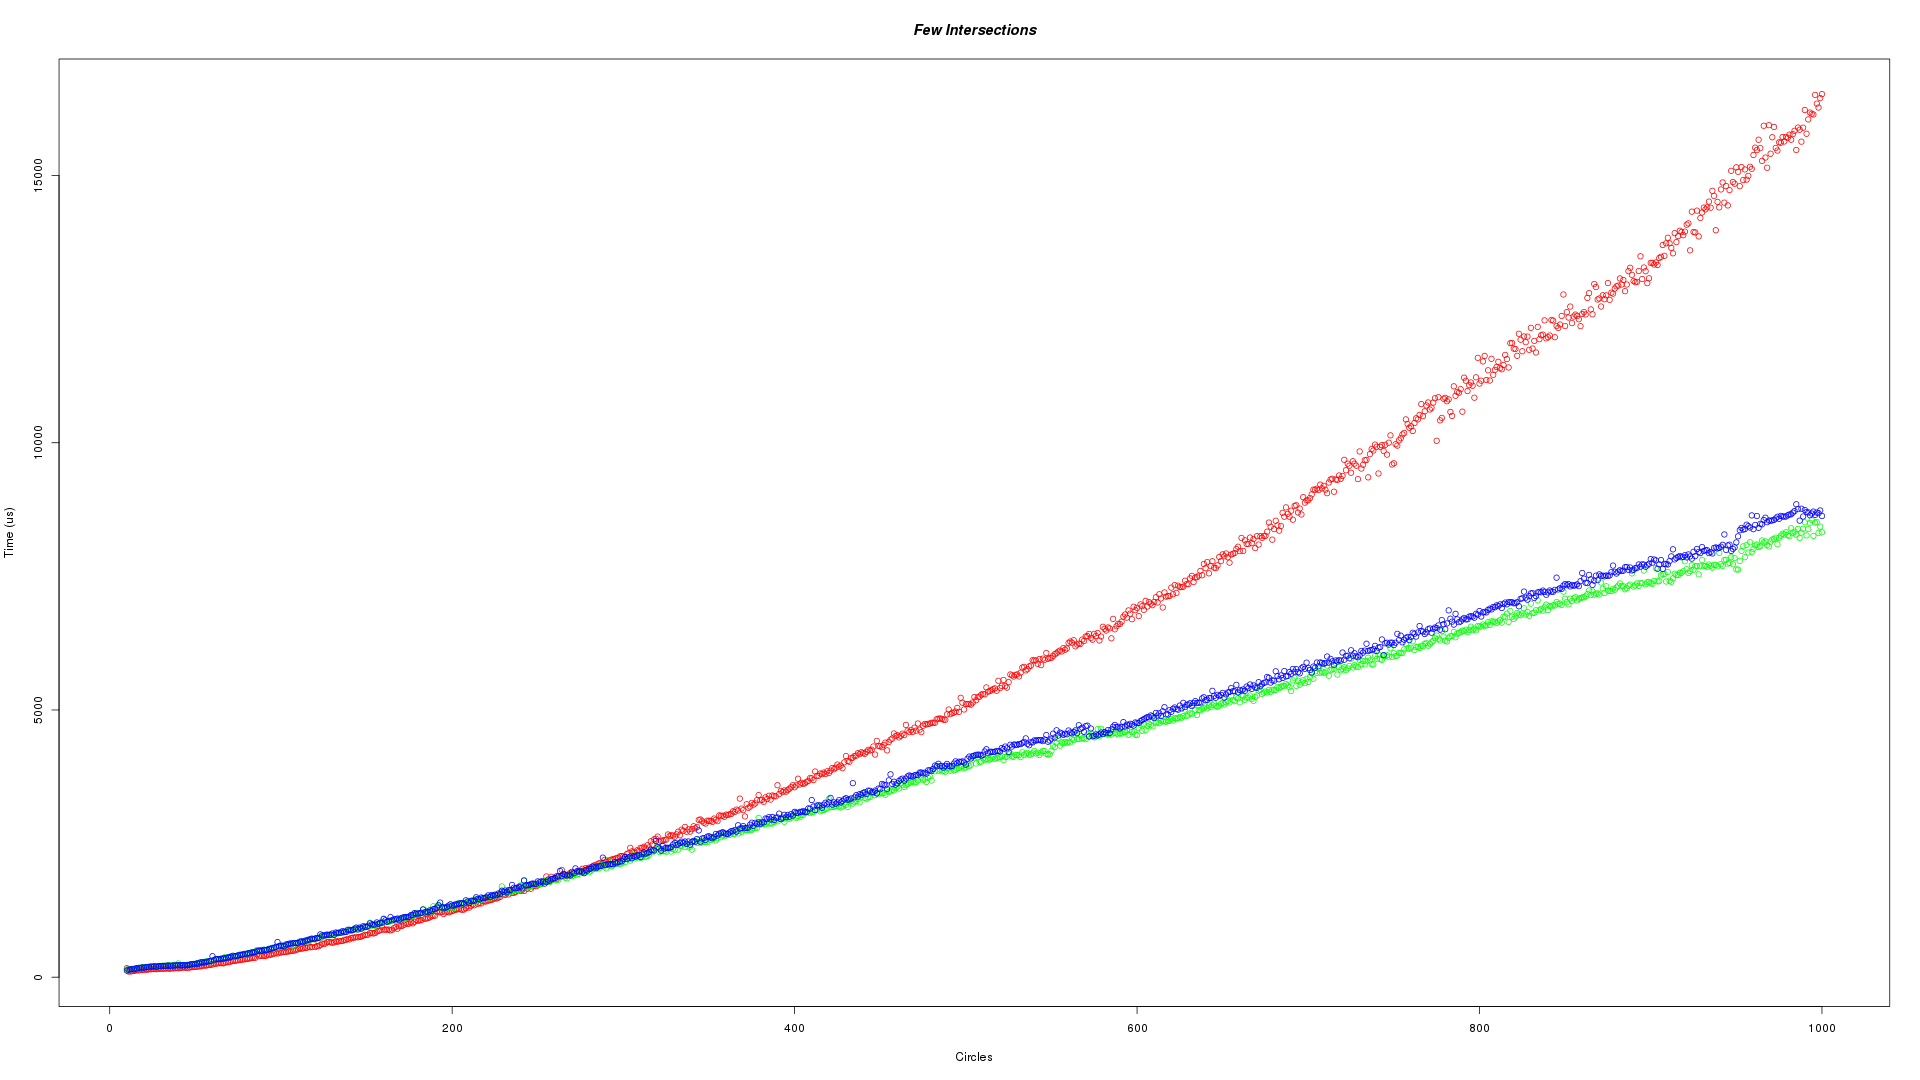
\includegraphics[width=\textwidth]{illustraties/fewIntersections.png}
  	\caption{Uitvoeringstijden bij gevallen met weinig snijpunten.}
  	\label{fig:few_intersections}
\end{figure}
In figuur \ref{fig:few_intersections} zijn de resultaten uiteengezet van het eerste rauwe data-experiment. We zien dat het na\"ieve algoritme veel slechter presteert dan de andere twee. Het eerste algoritme wordt niet be\"invloedt door het aantal snijpunten, lijkt het.

\subsubsection{Gemiddeld geval}
\begin{figure}[H]
	\centering
   	\includegraphics[width=\textwidth]{illustraties/averageCase.png}
  	\caption{Uitvoeringstijden bij een gemiddeld geval snijpunten.}
  	\label{fig:average_case}
\end{figure}
In figuur \ref{fig:average_case} zijn de resultaten uiteengezet voor een gemiddeld geval. We zien dat algoritme \'e\'en nog steeds ongeveer even snel werk. We zien ook dat algoritme twee en drie sneller zijn, zoals verwacht.
   
\subsubsection{Veel snijpunten}
\begin{figure}[H]
   	\centering
   	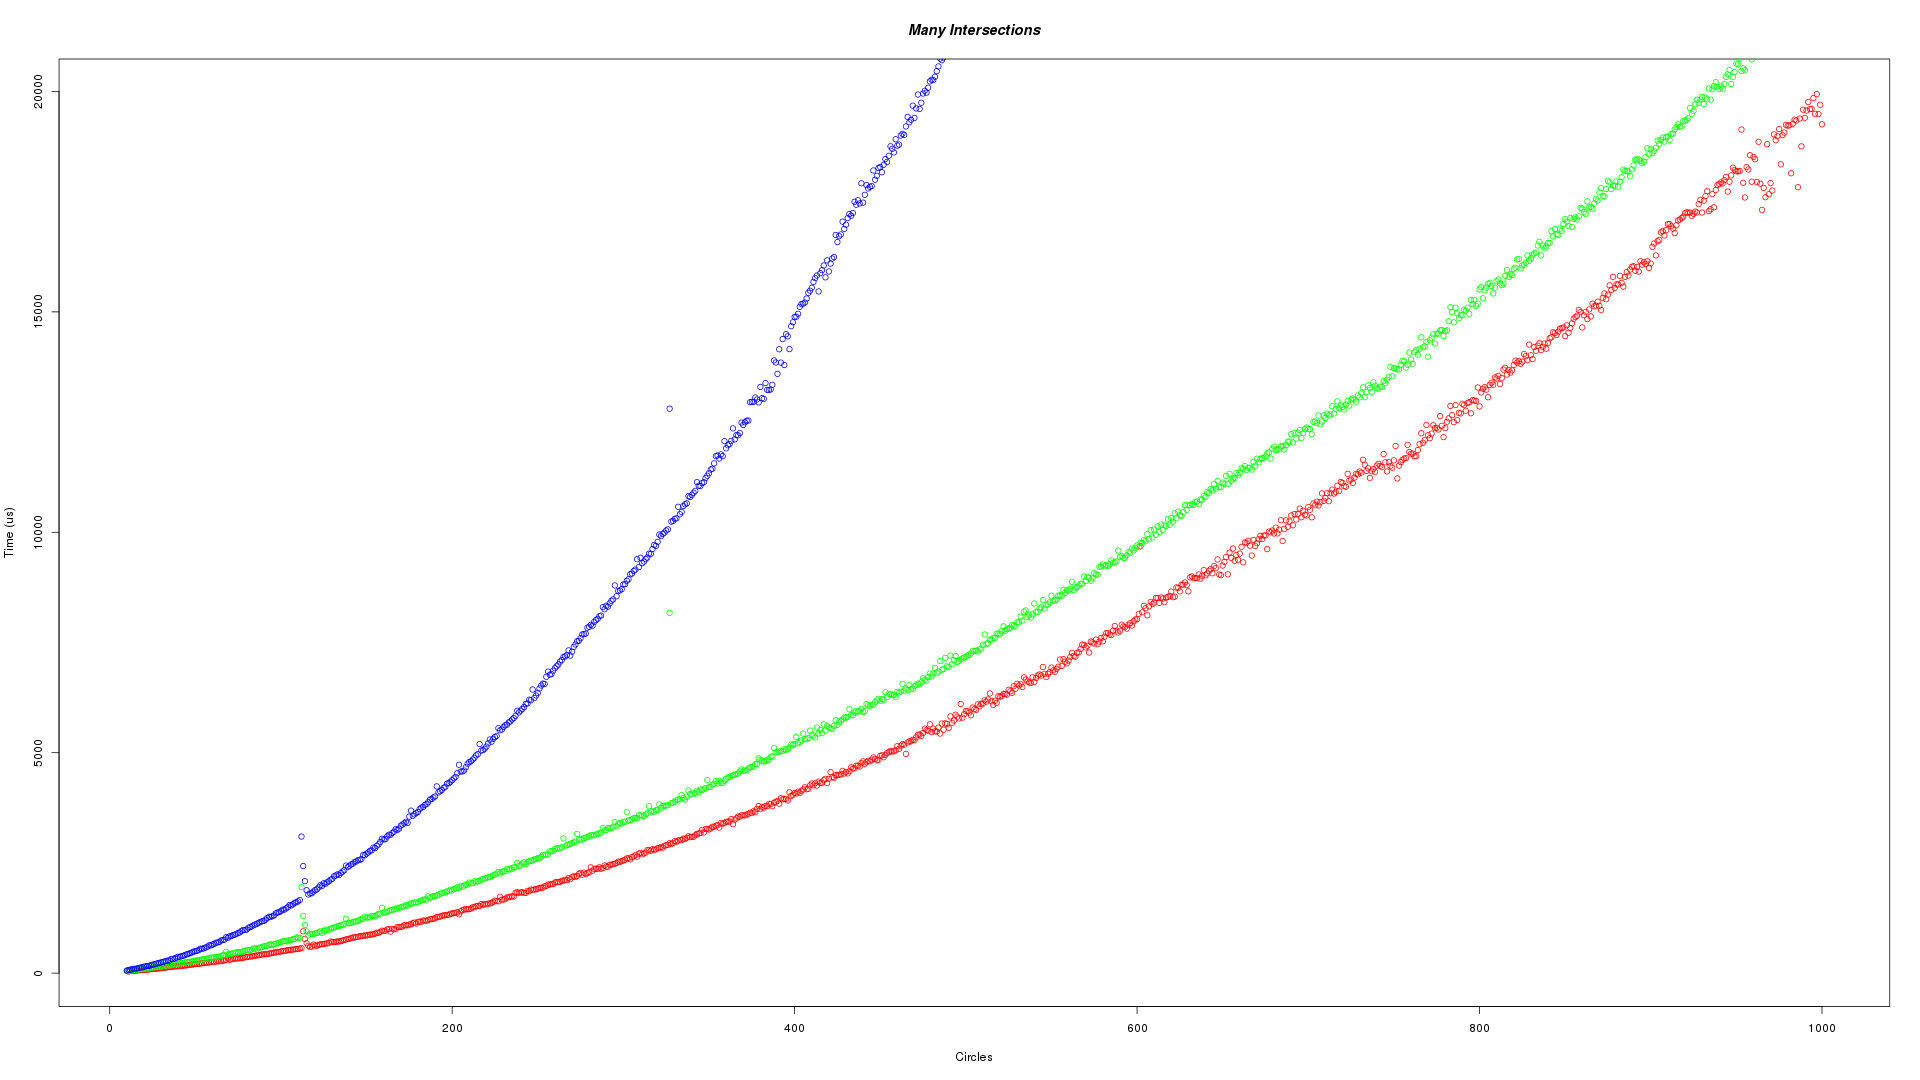
\includegraphics[width=\textwidth]{illustraties/manyIntersections.png}
  	\caption{Uitvoeringstijden bij gevallen met relatief veel snijpunten.}
   	\label{fig:many_intersections}
\end{figure}
In figuur \ref{fig:many_intersections} zijn de resultaten uiteengezet van het tweede rauwe data-experiment. We zien dat algoritme \'e\'en hier beter presteert dan de andere twee. Algoritme twee en drie moeten dezelfde snijpunten berekenen maar hebben te kampen met enige `overhead'.

\subsubsection{3D plot}
\begin{figure}[H]
   	\centering
   	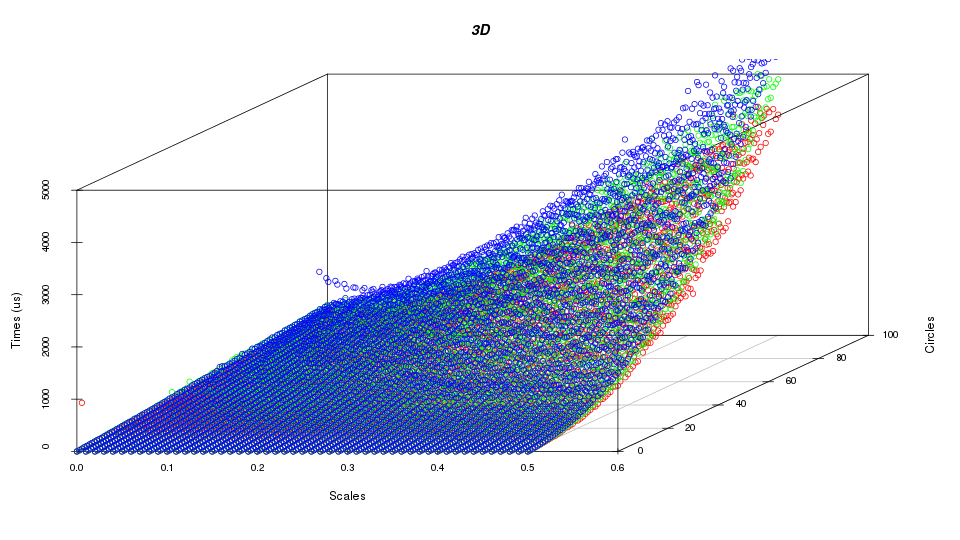
\includegraphics[width=\textwidth]{illustraties/3DScatter.png}
  	\caption{Een 3D grafiek van de uitvoeringstijden in functie van de scalering en het aantal cirkels}
	\label{fig:3d}
\end{figure}
De resultaten van het laatste rauwe data-experiment staan in figuur \ref{fig:3d}.
Het is duidelijk dat algoritme \'e\'en ongeveer evenveel tijd nodig heeft onafhankelijk van de scalering van de stralen. We zien bovendien dat algoritme drie slechter presteert dan algoritme \'e\'en bij grote scaleringen en beter bij kleine scaleringen.

\begin{figure}[H]
   	\centering
   	\includegraphics[width=\textwidth]{illustraties/3DnrIs.png}
  	\caption{Aantal snijpunten}
  	\label{fig:nr_intersections}
\end{figure}

In figuur \ref{fig:nr_intersections} staan het aantal snijpunten geplot voor elk geval, in plaats van de uitvoeringstijden. We zien dat de grafiek van de uitvoeringstijden van algoritme drie mooi dezelfde vorm heeft.

\subsection{Doubling ratio}
De resultaten van een doubling ratio experiment zetten we in een tabel. Op de bovenste rij van de tabel staat het aantal cirkels. In de meest linkse kolom staan de scaleringen van de straal. De getallen in de tabel stellen de verhouding voor tussen de uitvoeringstijd bij deze probleemgrootte ten opzichte van het probleemgrootte er links van.

\subsubsection{Naief}
\begin{table}[H]
\[
\begin{array}{|c||ccccccc|}
\hline 
& 20 & 40 & 80 & 160 & 320 & 640 & 1280\\
\hline \hline 
0.000 & 3.4 & 3.9 & 4.6 & 4.2 & 4.3 & 4.3 & 4.2 \\ \hline 
0.001 & 3.2 & 4.3 & 4.2 & 4.9 & 4.1 & 4.3 & 4.2 \\ \hline 
0.500 & 3.5 & 4.0 & 4.5 & 4.8 & 4.9 & 4.8 & 5.0 \\ \hline 
1.000 & 3.4 & 4.2 & 4.5 & 4.7 & 5.3 & 5.3 & 5.3 \\ \hline 
\end{array}
\]


\caption{Doubling ratio 1}
\label{fig:doublingratio_1}
\end{table}
tabel \ref{fig:doublingratio_1} toont de resultaten van het doubling ratio exeriment voor algoritme \'e\'en. Het is makkelijk te zien dat de ratio zal convergeren naar $4$ voor een groot aantal cirkels. Dit bovendien onafhankelijk van de scalering van de stralen. Wanneer er veel snijpunten zijn lijkt het algoritme last te hebben van enige overhead. We weten niet waarom, maar algoritme \'e\'en is zodanig eenvoudig dat we denken dat het probleem misschien bij Haskell zelf ligt.


\subsubsection{Kwadratisch}
\begin{table}[H]
\[
\begin{array}{|c||ccccccc|}
\hline 
& 20 & 40 & 80 & 160 & 320 & 640 & 1280\\
\hline \hline 
0.000 & 1.8 & 2.3 & 2.2 & 2.3 & 2.1 & 2.2 & 2.1 \\ \hline 
0.001 & 2.0 & 2.4 & 2.1 & 2.5 & 2.2 & 2.3 & 2.6 \\ \hline 
0.500 & 3.1 & 3.9 & 4.2 & 4.3 & 5.1 & 5.2 & 5.1 \\ \hline 
1.000 & 3.7 & 4.3 & 4.0 & 4.7 & 5.5 & 5.1 & 5.4 \\ \hline 
\end{array}
\]


\caption{Doubling ratio 2}
\label{fig:doublingratio_2}
\end{table}
In tabel \ref{fig:doublingratio_2} de resultaten van het doubling ratio experiment voor algoritme twee. Voor kleine scaleringen van de straal zien we dat de ratio rond $2.2$ schommelt. Wanneer er weinig snijpunten zijn is dit algoritme dus inderdaad beter dan kwadratisch.
Voor grote scaleringen zou de verhouding naar $4$ moeten gaan, maar ook deze erhoudingen lijken rond $5.2$ te schommelen. Opnieuw kunnen we niet verklaren waarom.

\subsubsection{Linearitmisch}
\begin{table}[h]
\[
\begin{array}{|c||ccccccc|}
\hline 
& 20 & 40 & 80 & 160 & 320 & 640 & 1280\\
\hline \hline 
0.000 & 2.2 & 2.2 & 2.2 & 2.3 & 2.2 & 2.1 & 2.2 \\ \hline 
0.001 & 2.1 & 2.2 & 2.2 & 2.3 & 2.8 & 1.8 & 2.4 \\ \hline 
0.500 & 3.3 & 3.4 & 4.1 & 4.4 & 5.2 & 5.2 & 5.0 \\ \hline 
1.000 & 3.4 & 4.0 & 4.2 & 4.6 & 5.5 & 5.1 & 5.1 \\ \hline 
\end{array}
\]


\caption{Doubling ratio 3}
\label{fig:doublingratio_3}
\end{table}
In tabel \ref{fig:doublingratio_3} staan de resultaten van het laatste doubling ratio experiment.
We zien dat de ratio rond $2.2$ schommelt voor kleine scaleringen.
Dit komt overeen met onze voorspellingen.
Bij kleine $S$ zal de uitvoeringstijd van het algoritme namelijk linearitmisch groeien.
Bij grote scaleringen schommelt de ratio boven $4$ zoals verwacht van een $O(N^2\log(N))$ algoritme. We weten echter niet of dit is omdat alles in orde is of omdat hetzelfde probleem zich stelt als bij de eerdere doubling ratio experimenten. Opnieuw zouden we geen verklaring hebben voor de verhoudingen die rond $5.1$ schommelen.

